\documentclass{article}
\usepackage[utf8]{inputenc}
\usepackage[margin = 0.8in]{geometry}
\usepackage{graphicx}
\usepackage{amsmath, amssymb}
\usepackage{subcaption}
\usepackage{multirow}
\usepackage{mathtools}
\usepackage{float}
\usepackage[linesnumbered,ruled]{algorithm2e}



\title{RBE595 - Week 13 Assignment}
\author{Keith Chester}
\date{Due date: April 24, 2023}

\begin{document}
\maketitle

\section*{Problem 1}
\textit{What are the two sources of error in Deep RL with function approximation?}

The two common sources are function approximation error and the sampling/estimation error.

When using neural nets to approximate value functions or policy functions in complex environments, the resulting neural net is a function approximation of the environment's true function. The difference is that there can be errors, biases, or edge cases not represented by the approximation. This can be combated by additional training, simulation, and more data depending on your approach; but in a sufficiently complex environment it may be possible that your net can never fully represent every possible situation.

Sampling/estimation error arises from having a too few samples to learn from in order to provide accurate representation. This is often cut off due to resource constraints - time, compute restraints, or sample inefficieny. An example of that last one could be operating in real space versus a simulation, preventing large scale collection of data.

\section*{Problem 2}
\textit{In TD learning with a neural network what are we trying to minimize? What are we trying to maximize?}

In temporal difference (TD) learning with neural networks we are aiming to minimize the error between the predicted and actual values of a particular state/action pair. Our primary goal is to maximize the ultimate reward we get from the agent by minimizing this error of prediction.


\section*{Problem 3}
\textit{What is the main benefit of deep neural networks in function approximation compared to linear method? What is the linear function approximation useful for?}

A linear method to solving a system involves creating a equation that directly describes the behavior of a system. From it we can quickly and efficiently generate agents to fit a system and solve it. Neural networks can approximate any function given a deep enough network, but require training in order to approximate a given system.

When a system is simple enough, a linear method of developing a linear equation is easily done and significantly more efficient to learn than any neural net. The problem is that systems that become more complex become harder to represent, until you reach a level of complexity where a neural net's ability to approximate any function becomes the only method efficient enough to represent and solve the system as an agent.

\section*{Problem 4}
\textit{In DQN, what is the purpose of the target network and value network?}

In Deep-Q Networks (DQN), the target network and value network are each a Q-function approximator hoping to correctly evaluate the value of a given state/action pair. The target network is used to generate the target values for the value network to train on. The target network is updated less frequently than the value network, and is used to generate the target values for the value network to train on. By having the two networks update separately and not in lockstep with eachother we have a more stable training process for our agent.

\section*{Problem 5}
\textit{In the Deep Q-learning method, which are true:}
\begin{itemize}
    \item \textbf{a}. \textit{epsilon-greedy is required to ensure exploration.}
    \item \textbf{b}. \textit{exploration this taken care of by the randomization provided by experience replay?}
\end{itemize}

Epislon-greedy is a method for determining and balancing choosing an action at random rather than choosing the greedy option of the best possible choice of an action presented to the agent at a given state. Experience replay is a method of training networks like DQNs that record momentary states and the resulting values/actions for the agent to repeatedly learn from.

Experience replay isn't strictly for exploration but more for stability of training through allowing the agent to avoid "forgetting" past experiences and situations. The random presentation of states and experiences from the agent's past can be viewed as a form of exploration, but does not allow the agent to choose new unexplored paths quite like epsilon-greedy would.

Thus I would argue that A is true between the two options presented.

\section*{Problem 6}
\textbf{True or False:} \textit{Value function-based RL methods are oriented towards finding deterministic policies whereaspolicy search methods are geared towards finding stochastic policies.}

This is true; when we are trying to find a value function we're hoping to create a deterministic and ultimately accurate function that gives us a numerical score for the value of a given state. Policies, however, are stochastic as they alow appropriate exploitation/exploration during training. Likewise, if we look at the popular method of dealing with continuous (versus discrete) action spaces, a popular method is to have networks generate the prerequisties for a distribution (such as mean and variance fed into a normal distribution) to create a stochastic policy for a given state.

\section*{Problem 7}
\textit{What makes the optimization space smooth in policy gradient methods?}

Policy gradient methods have smooth optimization spaces as they use differentiable policy functions. This allows us to use gradient descent to optimize the policy function and find the best possible policy for a given state. We also typically use a smooth objective function that measures the expected reward/return in which to optimize itself.

\section*{Problem 8}
\textit{How does actor-critic architecture improve the “vanila” policy gradient?}

Typical non actor-critic policy gradients ("vanilla") have high variance and unstable/noisy gradients. When a critic network is introduced it helps create a more stable and accurate gradient when its used to estimate the value of a given action taken by the actor model.

\section*{Problem 9}
\textit{What is the Advantage function, $A_\pi(s_t,a_t)$ in actor-critic architecture? Write down the
equation for monte-carlo-based Advantage function and TD-based advantage function and
comment on the pro and cons of each on.}

\subsection*{Monte Carlo Advantage}
\begin{equation}
    A(s,a) = \sum^T_{k=t+1} r(s^i_k, a^i_k ) - V_\pi(s^i_t)
\end{equation}
\textbf{Pros}
\begin{itemize}
    \item Low bias
\end{itemize}

\textbf{Cons}
\begin{itemize}
    \item Slow convergence
    \item Requires a full episode to conclude
    \item Suffers from high variance
\end{itemize}

\subsection*{TD Advantage Advantage}
\begin{equation}
    A(s,a) = r(s_{t+1}, a_{t+1}) + V_\pi(s_{t+1}) - V_\pi(s_t)
\end{equation}
\textbf{Pros}
\begin{itemize}
    \item Lower variance than Monte Carlo
    \item Faster convergence
    \item Updates on each step - doesn't require terminal episode to be reached
\end{itemize}

\textbf{Cons}
\begin{itemize}
    \item Higher bias
\end{itemize}

\section*{Problem 10}
\textit{Can you find a resemblance between actor-critic architecture and generalized policy iteration in
chapter 4?}

In both the actor-critic architecture and generalized policy iteration aim to improve its ability to evaluate a given policy (policy evaluation for GPI, the critic for value function), and their policy overall.

\section*{Problem 11}
\textit{In the actor-critic architecture described in the lecture, assuming the use of differentiable
function approximators, we can conclude that the use of such a scheme will result in:}
\begin{itemize}
    \item \textbf{A}. \textit{convergence to a globally optimal policy}
    \item \textbf{B}. \textit{convergence to a locally optimal policy}
    \item \textbf{C}. \textit{cannot comment on the convergence of such an algorithm}
\end{itemize}

The answer is \textbf{B} - the actor-critic architecture will find a locally optimal polcy, but is unlikely to find the globally optimal one. Still, it may be good enough for a given agent's performance.

\section*{Problem 12}
\textit{Assume that we are using the linear function approximation for the critic network and SoftMax policy with linear function approximation for the actor network. Write down the parameter update equations for the actor and the critic network (use on-line update equations similar to the algorithm in page 332)}

\subsection*{Actor Network Update}
\begin{equation}
    \sigma = R + \gamma \hat{v} (S,w) - \hat{v} (S,w)
\end{equation}
\begin{equation}
    w_{t+1} = w_t + \alpha^w \sigma \nabla \hat{v} (S,w)
\end{equation}

\subsection*{Critic Network Update}
\begin{equation}
    \theta = \theta + \alpha^\theta \sigma \nabla \pi_\theta (A | S)
\end{equation}
\begin{equation}
    I = \gamma I
\end{equation}

\section*{Problem 13}
\textit{Consider a trajectory rollout of $(s, a_1, s, a_2, s, a_3)$. The initial policy depicted in the figure below for state $s$.The horizontal line also shows the value of the Advantage function for each (state, action) pair. After applying the policy gradient update, what do you expect the probability of each action to change  to?}

\begin{figure}
    \centering
    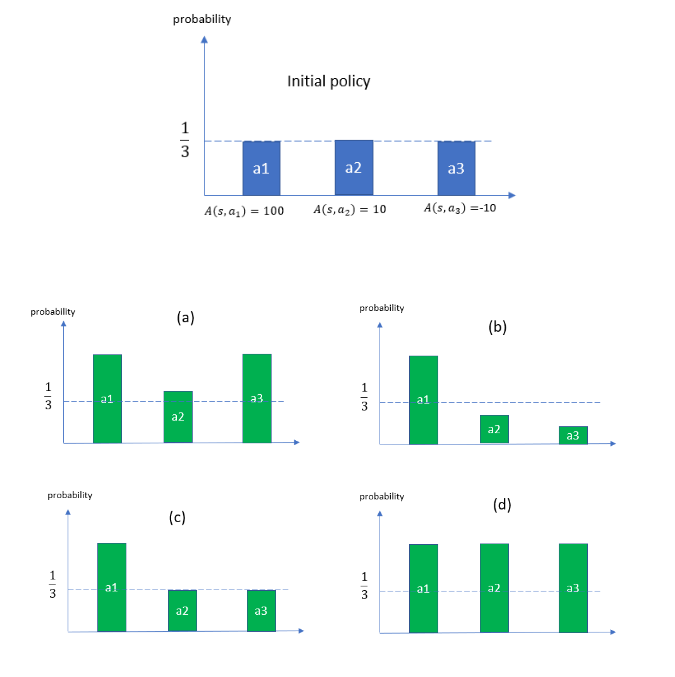
\includegraphics[width=.8\linewidth]{imgs/13.png}
    \caption{Problem 13 Options}
\end{figure}

The answer is \textbf{B}; we expect to see the probability for $a_1$ relative to $a_2$ and $a_3$ to increase sharply, resulting in decreases for the other two actions.



\end{document}